% Author: Izaak Neutelings (June 2017)
% taken from https://tex.stackexchange.com/questions/159445/draw-in-cylindrical-and-spherical-coordinates

\documentclass[border=3pt,tikz]{standalone}
\usepackage{physics}
\usepackage{tikz}
\usepackage{tikz-3dplot}
\usepackage[outline]{contour} % glow around text
\usepackage{xcolor}
\colorlet{veccol}{green!50!black}
\colorlet{projcol}{blue!70!black}
\colorlet{myblue}{blue!70!black}
\tikzset{>=latex} % for LaTeX arrow head
\tikzstyle{proj}=[projcol!80,line width=0.08] %very thin
\tikzstyle{area}=[draw=veccol,fill=veccol!80,fill opacity=0.6]
\tikzstyle{vector}=[->,veccol,thick]
\usetikzlibrary{angles,quotes} % for pic (angle labels)
\contourlength{1.3pt}

\begin{document}


% 3D AXIS with spherical coordinates
\tdplotsetmaincoords{60}{110}
\begin{tikzpicture}[scale=2,tdplot_main_coords]
  
  % VARIABLES
  \def\rvec{.8}
  \def\thetavec{30}
  \def\phivec{60}
  
  % AXES
  \coordinate (O) at (0,0,0);
  \draw[thick,->] (0,0,0) -- (1,0,0) node[anchor=north east]{$x$};
  \draw[thick,->] (0,0,0) -- (0,1,0) node[anchor=north west]{$y$};
  \draw[thick,->] (0,0,0) -- (0,0,1) node[anchor=south]{$z$};
  
  % VECTORS
  \tdplotsetcoord{P}{\rvec}{\thetavec}{\phivec}
  \draw[-stealth,red] (O)  -- (P) node[above right=-2] {P};
  \draw[dashed,red]   (O)  -- (Pxy);
  \draw[dashed,red]   (P)  -- (Pxy);
  \draw[dashed,red]   (Py) -- (Pxy);
  
  % ARCS
  \tdplotdrawarc[->]{(O)}{0.2}{0}{\phivec}
    {anchor=north}{$\phi$}
  \tdplotsetthetaplanecoords{\phivec}
  \tdplotdrawarc[->,tdplot_rotated_coords]{(0,0,0)}{0.4}{0}{\thetavec}
    {anchor=south west}{\hspace{-1mm}$\theta$}

\end{tikzpicture}


% 3D AXIS with spherical coordinates
\tdplotsetmaincoords{60}{110}
\begin{tikzpicture}[scale=1.8,tdplot_main_coords]
  
  % VARIABLES
  \def\l{0.3}
  \def\rvec{1.2}
  \def\thetavec{46}
  \def\phivec{50}
  
  % AXES
  \coordinate (O) at (0,0,0);
  \tdplotsetcoord{P}{\rvec}{\thetavec}{\phivec}
  \draw[dashed,myblue] (O)  -- (Pxy);
  \draw[thick,->] (0,0,0) -- (1,0,0) node[below left=-2]{$x$};
  \draw[thick,->] (0,0,0) -- (0,1,0) node[right=-1]{$y$};
  \draw[thick,->] (0,0,0) -- (0,0,1) node[above=-1]{$z$};
  \draw[vector] (0,0,0) -- (1.3*\l,0,0) node[above=3,left=-1,scale=0.8]{$\vu{x}$};
  \draw[vector] (0,0,0) -- (0,.9*\l,0) node[right=2,above=-1,scale=0.8]{$\vu{y}$};
  \draw[vector] (0,0,0) -- (0,0,\l) node[left,scale=0.8]{$\vu{z}$};
  
  % VECTORS
  \node[circle,inner sep=0.9,fill=myblue]
    (P') at ({\rvec*sin(\thetavec)*cos(\phivec)},{\rvec*sin(\thetavec)*sin(\phivec)},{\rvec*cos(\thetavec)}) {};
  \draw[-stealth,thick,myblue] (O)  -- (P') node[above right=-2] {P};
  \draw[dashed,myblue] (P)  -- (Pxy);
  \draw[dashed,myblue] (P)  -- (Pz);
  \draw[dashed,myblue] (Py) -- (Pxy) -- (Px);
  
  % ARCS
  \tdplotsetthetaplanecoords{\phivec}
  \tdplotdrawarc[->,tdplot_rotated_coords]{(0,0,0)}{0.4}{0}{\thetavec}
    {right=2,above}{$\theta$}

\end{tikzpicture}


% 3D AXIS with spherical coordinates, dA
\tdplotsetmaincoords{60}{103}
\begin{tikzpicture}[scale=2.8,tdplot_main_coords]
  
  % VARIABLE
  \def\rvec{1.0}
  \def\thetavec{35}
  \def\phivec{45}
  \def\dtheta{10}
  \def\dphi{16}
  \def\sphere#1#2#3{plot[domain=#1]({\rvec*sin(#2)*cos(#3)},{\rvec*sin(#2)*sin(#3)},{\rvec*cos(#2)})}
  
  % AXES
  \coordinate (O) at (0,0,0);
  \draw[thick,->] (0,0,0) -- (1.16*\rvec,0,0) node[left=2,below]{$x$};
  \draw[thick,->] (0,0,0) -- (0,1.1*\rvec,0) node[below=2,right=0]{$y$};
  \draw[thick,->] (0,0,0) -- (0,0,1.1*\rvec) node[above]{$z$};
  
  % COORDINATES
  \tdplotsetcoord{P}{\rvec}{\thetavec}{\phivec}
  \tdplotsetcoord{PB}{\rvec}{\thetavec+\dtheta}{\phivec}
  \tdplotsetcoord{PR}{\rvec}{\thetavec}{\phivec+\dphi}
  \tdplotsetcoord{PBR}{\rvec}{\thetavec+\dtheta}{\phivec+\dphi}
  
  % CONE
  \draw[veccol!10,very thin] (O)  -- (PBR);
  \draw[veccol!10,very thin] (O)  -- (PR);
  \draw[->,veccol] (O)  -- (P) node[below=5,left=2] {$\vb{r}$};
  \draw[veccol,very thin] (O)  -- (PB);
  
  % PROJECTIONS
  \draw[proj] %\thetavec+\dtheta
    plot[domain=0:90]({\rvec*sin(\x)*cos(\phivec)},{\rvec*sin(\x)*sin(\phivec)},{\rvec*cos(\x)}) coordinate (BL);
  \draw[proj]
    plot[domain=0:90]({\rvec*sin(\x)*cos(\phivec+\dphi)},{\rvec*sin(\x)*sin(\phivec+\dphi)},{\rvec*cos(\x)}) coordinate (BR);
  \draw[proj]
    plot[domain=0:90]({\rvec*cos(\x)},{\rvec*sin(\x)},0);
  \draw[proj] (O)  -- (BL); % PBxy
  \draw[proj] (O)  -- (BR); % PBRxy
  \draw[proj] (P)  -- (Pz);
  \draw[proj] (PR)  -- (Pz) node[midway,above=-2,rotate=-24] {\contour{white}{$r\sin\theta$}};
  %\draw[proj,projcol!15,dashed] (P) -- (Pxy);
  %\draw[proj,projcol!15,dashed] (PR) -- (PRxy);
  %\draw[proj,projcol!15,dashed] (PB) -- (PBxy);
  %\draw[proj,projcol!15,dashed] (PBR) -- (PBRxy);
  
  % AREA
  \draw[area]
    plot[domain=0:.99*\dphi]({\rvec*sin(\thetavec)*cos(\phivec+\x)},{\rvec*sin(\thetavec)*sin(\phivec+\x)},{\rvec*cos(\thetavec)}) --
    plot[domain=0:.99*\dtheta]({\rvec*sin(\thetavec+\x)*cos(\phivec+\dphi)},{\rvec*sin(\thetavec+\x)*sin(\phivec+\dphi)},{\rvec*cos(\thetavec+\x)}) --
    plot[domain=.99*\dphi:0]({\rvec*sin(\thetavec+\dtheta)*cos(\phivec+\x)},{\rvec*sin(\thetavec+\dtheta)*sin(\phivec+\x)},{\rvec*cos(\thetavec+\dtheta)}) --
    plot[domain=.99*\dtheta:0]({\rvec*sin(\thetavec+\x)*cos(\phivec)},{\rvec*sin(\thetavec+\x)*sin(\phivec)},{\rvec*cos(\thetavec+\x)}) --
    cycle;
    
  % MEASURES
  %\node[right=3,below right=-2] at (PB) {$r\sin\theta\dd{\phi}$};
  %\node[right=5,below right=-2] at (PR) {$r\dd{\theta}$};
  \draw[<->,proj,thin]
    plot[domain=0:\dphi]({\rvec*sin(\thetavec+1.11*\dtheta)*cos(\phivec+\x)},{\rvec*sin(\thetavec+1.11*\dtheta)*sin(\phivec+\x)},{\rvec*cos(\thetavec+1.11*\dtheta)})
    node[right=12,below] {\contour{white}{$r\sin\theta\dd{\phi}$}};
  \draw[<->,proj,thin]
    plot[domain=0:\dtheta]({\rvec*sin(\thetavec+\x)*cos(\phivec+1.15*\dphi)},{\rvec*sin(\thetavec+\x)*sin(\phivec+1.15*\dphi)},{\rvec*cos(\thetavec+\x)}) 
    node[above=11,right=-3] {$r\dd{\theta}$};
    
  % ANGLES
  \tdplotdrawarc[->]{(O)}{0.35*\rvec}{0}{\phivec}
    {anchor=north}{$\phi$}
  \tdplotdrawarc[->]{(O)}{0.45*\rvec}{\phivec}{\phivec+\dphi}
    {above=0.5,anchor=123}{\contour{white}{$\dd{\phi}$}}
  \tdplotsetthetaplanecoords{\phivec}
  \tdplotdrawarc[->,tdplot_rotated_coords]{(0,0,0)}{0.36*\rvec}{0}{\thetavec}
    {right=3,above}{$\theta$}
  \tdplotdrawarc[->,tdplot_rotated_coords]{(0,0,0)}{0.54*\rvec}{\thetavec}{\thetavec+\dtheta}
    {above right=-2}{\contour{white}{$\dd{\theta}$}}
  
\end{tikzpicture}


% SOLID ANGLE SURFACE INTEGRATION
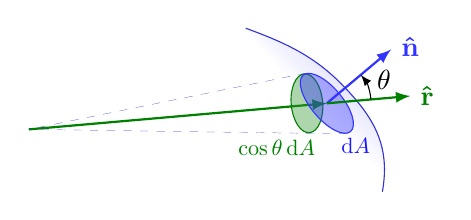
\begin{tikzpicture}
  
  % VARIABLE
  \def\R{3.8}
  \def\ang{5}
  \def\angII{40}
  \coordinate (O) at (0,0);
  \coordinate (P) at (\ang:\R);
  \coordinate (Pr) at (\ang:\R-0.25);
  
  % SURFACE
  \draw[blue!80!black!80,top color=white,bottom color=blue!20,middle color=white,shading angle=\angII+95]
    (\ang+20:0.8*\R) to[out=-20,in=130] (\ang:1.1*\R) to[out=-50,in=80] (\ang-15:1.2*\R);
  
  % CONE
  \draw[vector]
    (0,0) -- (P); % node[left=3,below left=2] {$\vb{r}$};
  %\begin{scope}
  %  \clip[shift={(P)},rotate around={22:(P)}]
  %    (-0.4,0) rectangle ++(0.8,0.8) -- cycle;
  %  \draw[draw=blue!80,fill=blue!80,fill opacity=0.6,rotate around={\angII:(P)},fill opacity=0.4]
  %    (P) ellipse (0.2 and 0.4);
  %\end{scope}
  \draw[area,fill opacity=0.4,rotate around={\ang:(Pr)}]
    (Pr)++(90+\ang:0.006*\R) ellipse (0.2 and 0.375);
  \draw[draw=blue!80,fill=blue!80,fill opacity=0.4,rotate around={\angII:(P)}]
    (P) ellipse (0.2 and 0.468);
  %\begin{scope}
  %  \clip[shift={(P)},rotate around={22:(P)}]
  %    (-0.4,0) rectangle ++(0.8,-0.8) -- cycle;
  %  \draw[draw=blue!80,fill=blue!80,fill opacity=0.6,rotate around={\angII:(P)},fill opacity=0.4]
  %    (P) ellipse (0.2 and 0.4);
  %\end{scope}
  \draw[dashed,proj]
    (P)++(\angII+84:0.464) coordinate (PT) -- (0,0);
  \draw[dashed,proj]
    (P)++(\angII-96:0.468) coordinate (PB) node[blue!90,right=3,below=-1,scale=0.8] {$\dd{A}$} -- (0,0);
  \node[veccol,left=11,below=10,scale=0.8] at (Pr) {$\cos\theta\dd{A}$};
  
  % VECTORS
  \draw[vector,blue!80]
    (P) --++ (\angII:0.28*\R) coordinate (N) node[above=1,right] {$\vu{n}$};
  \draw[vector]
    (P) --++ (\ang:0.28*\R) coordinate (R) node[right] {$\vu{r}$};
  \draw pic[->,"$\theta$",draw=black,angle radius=16,angle eccentricity=1.4] {angle = R--P--N};
  %\draw pic[->,"$\Delta\Omega$",draw=black,angle radius=26,angle eccentricity=1.4] {angle = PB--O--PT};
  
\end{tikzpicture}


\end{document}